\section{Definições de Requisitos Ágeis}
	
	\subsection{Requisitos Funcionais}

		\subsubsection{Nível de Portfólio}

			De acordo com o \textit{SAFe}, a visão de portfólio é responsável pelo alinhamento da estratégia de negócios da organização e intenções de investimento. Nela constam os temas de investimentos, os épicos de negócio e de arquitetura (LEFFINGWELL, 2010). 

			\begin{itemize}
			{
				\item Tema de Investimento:\\
				O tema de investimento identificado através do processo \textit{TO-BE} foi:
				\begin{itemize}
				{
					\item \textbf{TI}: Pesquisa de Mercado\\
				}
				\end{itemize}

				\item Épicos:\\
				Os épicos associados ao tema de investimento são:
				\begin{itemize}
				{
					\item \textbf{E-1}: Roteiro de Pesquisa\\

					\item \textbf{E-2}: Aplicação de QP\\

					\item \textbf{E-3}: Controle de Usuários\\
				}
				\end{itemize}
			}
			\end{itemize}


		\subsubsection{Nível de Programa}

			O nível de programa é responsável pelo gerenciamento das releases e dos recursos, identificação e priorização das \textit{features}, visando entrega contínua de valor para o cliente (LEFFINGWELL, 2010).

			\begin{itemize}
			{
				\item \textit{Features}:\\
				As \textit{features} derivadas do \textbf{E-1} são:
				\begin{itemize}
				{
					\item \textbf{FEAT-1.1}: Manutenção de DRP.\\

					\item \textbf{FEAT-1.2}: Manutenção de PRP.\\

					\item \textbf{FEAT-1.3}: Validação de PRP.\\

					\item \textbf{FEAT-1.4}: Manutenção de QP.\\
				}
				\end{itemize}

				As \textit{features} derivadas do \textbf{E-2} são:
				\begin{itemize}
				{
					\item \textbf{FEAT-2.5}: Resposta de QP.\\

					\item \textbf{FEAT-2.6}: Geração de Relatório Semântico.\\

					\item \textbf{FEAT-2.7}: Geração de Relatório Estatístico.\\
				}
				\end{itemize}

				A \textit{feature} derivada do \textbf{E-3} foi:
				\begin{itemize}
				{
					\item \textbf{FEAT-3.8}: Manutenção de Usuários.\\
				}
				\end{itemize}
			}
			\end{itemize}

		\subsubsection{Nível de Time}

			No nível de time, as equipes são organizadas de acordo com suas competências e habilidades para atender às demandas do projeto. Ocorrerá a definição das histórias de usuários, tarefas e serão realizadas iterações para a entrega de software. (LEFFINGWELL, 2010).

			\begin{itemize}
			{
				\item Histórias de Usuário:\\
				As histórias de usuário derivadas da \textbf{FEAT-1.1} são:
				\begin{itemize}
				{
					\item \textbf{US-1.1.1}: Eu, como Especialista de \textit{Marketing}, desejo criar uma DRP para o Especialista de Mercado desenvolver a PRP.\\
					Critérios de Aceitação:
						\begin{enumerate}
						{
							\item Deverá possuir o campo \textbf{Nome};
							\item Deverá possuir o campo \textbf{Descrição}.
						}
						\end{enumerate}

					\item \textbf{US-1.1.2}: Eu, como Especialista de \textit{marketing}, desejo atribuir uma DRP à um Especialista de Mercado para que ele possa visualizar a DRP.\\
					Critérios de Aceitação:
						\begin{enumerate}
						{
							\item Deverá ser possível visualizar uma lista de Especialista de Mercado disponíveis;
							\item Deverá ser possível selecionar um Especialista de Mercado como responsável por uma demanda de roteiro de pesquisa;
							\item O sistema deverá apresentar uma mensagem caso o Especialista de Mercado selecionado já esteja responsável por outra demanda de roteiro de pesquisa.
						}
						\end{enumerate}

					\item \textbf{US-1.1.3}: Eu, como Especialista de \textit{marketing}, desejo alterar uma DRP para poder atualizar suas informações.\\
					Critérios de Aceitação:
						\begin{enumerate}
						{
							\item Deverá ser possível cancelar a DRP;
							\item O sistema deverá apresentar uma mensagem de confirmação de cancelamento da DRP;
							\item Deverá ser possível alterar o nome e a descrição da DRP;
							\item Deverá ser possível alterar o responsável pela DRP através de uma lista de Especialista de Mercado disponíveis;
							\item O sistema deverá apresentar uma mensagem de confirmação de alteração do responsável pela DRP.\\
						}
						\end{enumerate}

					\item \textbf{US-1.1.4}: Eu, como Especialista de \textit{marketing}, desejo importar arquivos do projeto para que a DRP contenha informações do projeto.\\
					Critérios de Aceitação:
						\begin{enumerate}
						{
							\item O sistema deverá apresentar a opção de adicionar arquivos durante a criação e alteração de uma DRP;
							\item Deverá ser possível importar arquivos do tipo: Imagem(JPEG, PNG), documentos (.docx, .pdf, .xls) e arquivos (.zip, .rar);
							\item Caso um dos arquivos seja uma imagem, deve-se criar uma galeria de imagem para visualização;
							\item Caso um dos arquivos seja documento, o mesmo deve estar disponível para download.
							\item Os itens só poderão ser modificados se exigida a devida correção;
							\item Caso o arquivo seja do tipo .zip ou .rar, deve-se descompactá-lo para que o acesso ao conteúdo seja possível.\\
						}
						\end{enumerate}

				}
				\end{itemize}



				As histórias de usuário derivadas da \textbf{FEAT-1.2} são:
				\begin{itemize}
				{
					\item \textbf{US-1.2.5}: Eu, como Especialista de Mercado, desejo manter os tópicos da PRP para construir uma PRP.\\
					Critérios de Aceitação:
						\begin{enumerate}
						{
							\item Deverá possuir os campos: Descrição, categoria, observação e referências;
							\item Ao deletar um tópico, deve-se pedir confirmação ao usuário;
							\item Não pode-se alterar nem deletar tópicos aprovados.\\
						}
						\end{enumerate}

					\item \textbf{US-1.2.6}: Eu, como Especialista de Mercado, desejo referenciar tópicos para criar uma relação entre eles.\\
					Critérios de Aceitação:
						\begin{enumerate}
						{
							\item Durante a criação ou alteração de um tópico deve-se poder visualizar uma lista de tópicos da mesma categoria;
							\item Deve-se poder selecionar um ou mais tópicos da lista para referenciá-los entre si.\\
						}
						\end{enumerate}

					\item \textbf{US-1.2.7}: Eu, como Especialista de Mercado, desejo submeter o tópico da PRP para solicitar a aprovação do tópico da PRP.\\
					Critérios de Aceitação:
						\begin{enumerate}
						{
							\item Para poder submeter um tópico deve ser preenchido ao menos o descrição e categoria;
							\item Deve-se ter um aviso de confirmação;
							\item Deve-se congelar um tópico que já foi enviado;
							\item Ser possível visualizar o status do tópicos.\\
						}
						\end{enumerate}
				}
				\end{itemize}



				As histórias de usuário derivadas da \textbf{FEAT-1.3} são:
				\begin{itemize}
				{
					\item \textbf{US-1.3.8}: Eu, como Especialista de \textit{marketing}, desejo aprovar o tópico submetido da PRP para consolidar o RP.\\
					Critérios de Aceitação:
						\begin{enumerate}
						{
							\item Deve ser possível visualizar os tópicos submetidos;
							\item Deve ser possível escolher entre as opções de aprovar e reprovar um tópico de PRP;
							\item Ao se aprovar todos os tópicos deve-se mostrar um aviso ao usuário mostrando que o RP foi consolidado;
							\item Ao reprovar um tópico deve-se mostrar uma mensagem de confirmação ao usuário;
							\item Tópicos reprovados devem deixar de serem visualizados pelo EMA;
							\item Deve-se exigir um comentário de justificativa ao reprovar um tópico.\\
						}
						\end{enumerate}


					\item \textbf{US-1.3.9}: Eu, como Especialista, desejo incluir comentários para discutir sobre o tópico de PRP.\\
					Critérios de Aceitação:
						\begin{enumerate}
						{
							\item Deve-se poder incluir comentários a qualquer momento;
							\item O comentário deve possuir o nome de quem o enviou, a data e o horário de envio;
							\item Os comentários devem ser mostrados em ordem temporal (o mais recente no topo).
						} 
						\end{enumerate}
				}
				\end{itemize}



				As histórias de usuário derivadas da \textbf{FEAT-1.4} são:
				\begin{itemize}
				{
					\item \textbf{US-1.4.10}: Eu, como Especialista, desejo criar questões de um tópico do RP para construir o QP.\\

					\item \textbf{US-1.4.11}: Eu, como Especialista, desejo votar em uma questão para consolidar o QP.\\

					\item \textbf{US-1.4.12}: Eu, como Especialista, desejo incluir comentários para discutir sobre a questão do QP.\\

					\item \textbf{US-1.4.13}: Eu, como Especialista de \textit{marketing} criador da DRP, desejo ordenar as questões aprovadas para concluir o QP.\\
				}
				\end{itemize}



				As histórias de usuário derivadas da \textbf{FEAT-2.5} são:
				\begin{itemize}
				{
					\item \textbf{US-2.5.14}: Eu, como Especialista de \textit{marketing}, desejo ajustar configurações da aplicação do QP para iniciar sua aplicação.\\

					\item \textbf{US-2.5.15}: Eu, como entrevistado, desejo responder o QP disponível para registrar minhas  informações no QP.\\
				}
				\end{itemize}



				As histórias de usuário derivadas da \textbf{FEAT-2.56} são:
				\begin{itemize}
				{
					\item \textbf{US-2.6.16}: Eu, como Especialista, desejo visualizar as informações respondidas do questionário para obter conhecimento das respostas.\\

					\item \textbf{US-2.6.17}: Eu, como Especialista, desejo analisar temporalmente as respostas dos QP, para obter conhecimento da frequência das respostas.\\

					\item \textbf{US-2.6.18}: Eu, como Especialista, desejo visualizar uma análise quantitativa, para obter conhecimento da estatística das respostas do QP.\\
					Referência: E-2, FEAT-2.6.

					\item \textbf{US-2.6.19}: Eu, como Especialista, desejo visualizar os gráficos das respostas para obter conhecimento da estatística das respostas do QP.\\
					Referência: E-2, FEAT-2.6.
				}
				\end{itemize}



				As histórias de usuário derivadas da \textbf{FEAT-2.7} são:
				\begin{itemize}
				{
					\item \textbf{US-2.7.20}: Eu, como Especialista, desejo visualizar as informações respondidas do questionário para obter conhecimento das respostas.\\

					\item \textbf{US-2.7.21}: Eu, como Especialista, desejo analisar temporalmente as respostas dos QP, para obter conhecimento da frequência das respostas.\\

					\item \textbf{US-2.7.22}: Eu, como Especialista, desejo visualizar uma análise quantitativa, para obter conhecimento da estatística das respostas do QP.\\

					\item \textbf{US-2.7.23}: Eu, como Especialista, desejo visualizar os gráficos das respostas para obter conhecimento da estatística das respostas do QP.\\
				}
				\end{itemize}


				
				As histórias de usuário derivadas da \textbf{FEAT-3.8} são:
				\begin{itemize}
				{
					\item \textbf{US-3.8.24}: Eu, como Especialista, desejo analisar temporalmente as respostas dos QP, para obter conhecimento da frequência das respostas.\\
					Referência: E-3, FEAT-3.8.

					\item \textbf{US-3.8.25}: Eu, como Especialista, desejo analisar temporalmente as respostas dos QP, para obter conhecimento da frequência das respostas.\\
					Referência: E-3, FEAT-3.8.

					\item \textbf{US-3.8.26}: Eu, como Especialista, desejo analisar temporalmente as respostas dos QP, para obter conhecimento da frequência das respostas.\\
					Referência: E-3, FEAT-3.8.

					\item \textbf{US-3.8.26}: Eu, como Especialista, desejo analisar temporalmente as respostas dos QP, para obter conhecimento da frequência das respostas.\\
					Referência: E-3, FEAT-3.8.
				}
				\end{itemize}
			}
			\end{itemize}


	\subsection{Requisitos Não-Funcionais}

		Requisitos não-funcionais são requisitos que expressam uma qualidade que o software deve ter. Diferencia-se dos requisitos funcionais por não referenciar funcionalidades do sistema, e sim comportamento ou restrição necessária para que a aplicação seja considerada satisfatória pelo cliente (DUARTE, 2002).

		\vspace*{0.5cm}

		\begin{table}[htbp]
			\caption{Tabela de Requisitos Não-Funcionais}
			\begin{tabular}{|l|l|p{11cm}|}
				\hline
				 & \textbf{Tipo} & \textbf{Descrição} \\ \hline
				\textbf{RNF01} & Usabilidade  & O sistema deve ser fácil de usar, sendo intuitivo, eficiente, permitindo o rápido acesso às funcionalidades do sistema e utilizar padrões de usabilidade. \\ \hline

				\textbf{RNF02} & Segurança & O sistema deve ser seguro, não divulgando informações do usuário e restringir o acesso requisitando login e senha. \\ \hline

				\textbf{RNF03} & Performance & O sistema deve responder às operações realizadas em, no máximo, 3 segundos. \\ \hline
			\end{tabular}
		\label{Tabela de Requisitos Não-Funcionais}
		\end{table}


	\subsection{Rastreabilidade}

	A rastreabilidade auxilia a engenharia de requisitos no controle dos requisitos, elementos de modelagem e outros artefatos do processo de software. Por meio dela, é possivel obter visualizar de onde surgiu tal requisito, quais são suas dependências e ainda quais deles serão afetados quando houver algum tipo de mudança.

	No desenvolver deste projeto será utilizado dois tipos de rastreabildade, a vertical e a horizontal.
	
	\subsubsection{Rastreabilidade Vertical}
	A rastreabilidade vertical será utilizada no projeto para identificar a origem dos requisitos, ela está presente nas relações de um nível de abstração e outro.\\

		\begin{figure}[!htp]
			\centering
			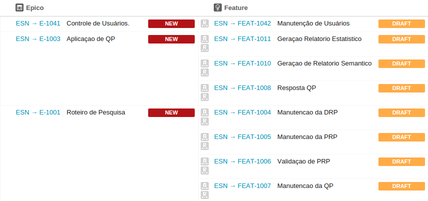
\includegraphics{imagens/epicfeat.png}
			\caption{Rastreabilidade vertical de epicos e \textit{features}.}
			\label{imagem}
		\end{figure}

		\begin{figure}[!htp]
			\centering
			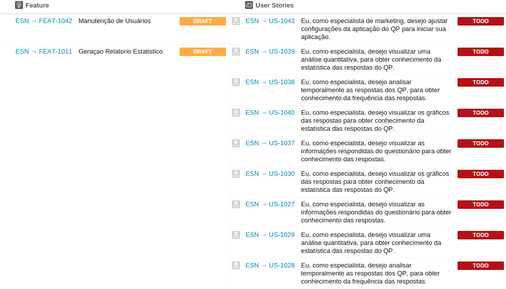
\includegraphics{imagens/featus.png}
			\caption{Rastreabilidade vertical de \textit{features} e histórias de usuário.}
			\label{imagem}
		\end{figure}

		\begin{figure}[!htp]
			\centering
			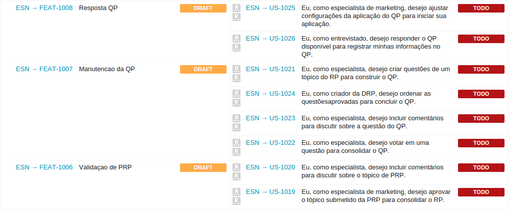
\includegraphics{imagens/featus2.png}
			\caption{Rastreabilidade vertical de \textit{features} e histórias de usuário.}
			\label{imagem}
		\end{figure}

		\begin{figure}[!htp]
			\centering
			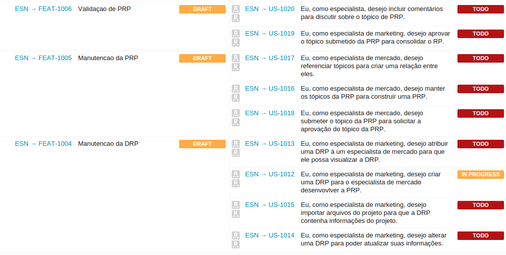
\includegraphics{imagens/featus3.png}
			\caption{Rastreabilidade vertical de \textit{features} e histórias de usuário.}
			\label{imagem}
		\end{figure}

	\newpage
	\subsubsection{Rastreabilidade Horizontal}
	A rastreabilidade horizontal será utilizada no projeto para identificar as dependencias entre um requisito e outro de um mesmo nível de abstração.\\

		\begin{figure}[!htp]
			\centering
			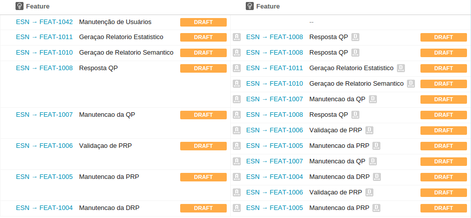
\includegraphics{imagens/featfeat.png}
			\caption{Rastreabilidade horizontal entre \textit{features}.}
			\label{imagem}
		\end{figure}